\documentclass[11pt]{standalone}
\usepackage{amssymb}
\usepackage{amsmath}
\usepackage[no-math]{fontspec}
\usepackage{unicode-math}
\usepackage{libertinus}
\usepackage{pgf,xcolor}
\usepackage{tikz}
\usetikzlibrary{arrows.meta, backgrounds}
\usepackage{pgfplots}
\pgfplotsset{compat=newest}

\definecolor{my_darkgray}{HTML}{484949}
\definecolor{my_lightgray}{HTML}{F3F4F4}
\definecolor{my_darkblue}{HTML}{005A94}
\definecolor{my_lightblue}{HTML}{CCDEE9}
\definecolor{my_yellow}{HTML}{FFEC7F}
\definecolor{my_red}{HTML}{E60000}
\definecolor{my_orange}{HTML}{E87846}

\begin{document}
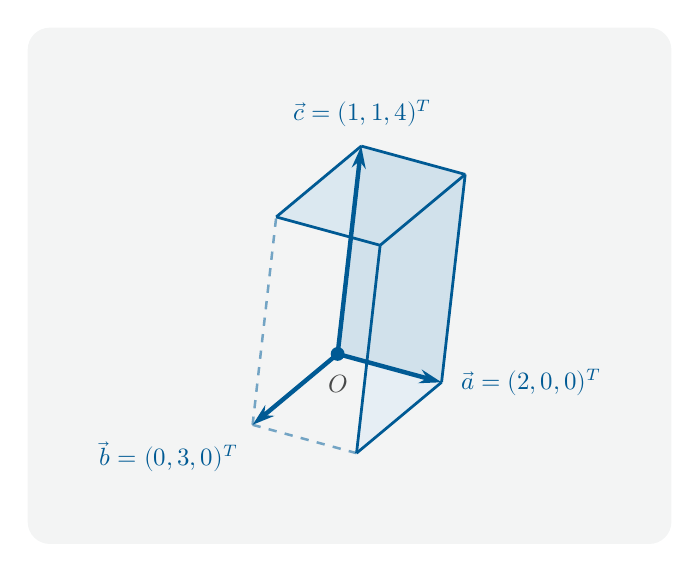
\begin{tikzpicture}[
    show background rectangle,
    background rectangle/.style={fill=my_lightgray, rounded corners=8pt},
    inner frame sep=0.8cm
]

% ---------------------------------------------------------------
%  Oblique projection of the parallelepiped spanned by
%    a = (2, 0, 0),   b = (0, 3, 0),   c = (1, 1, 4)
%
%  Projection rule:
%    (x, y, z)  -->  (0.66 x - 0.36 y,  -0.18 x - 0.30 y + 0.78 z)
%
%  Visible faces (viewing from front-right-above):
%    Front face  O -- vA -- vAC -- vC
%    Top face    vC -- vAC -- vABC -- vBC
%    Right face  vA -- vAB -- vABC -- vAC
%  Hidden vertex: vB (three incident edges drawn dashed)
% ---------------------------------------------------------------

\coordinate (O)    at ( 0.00,  0.00);   %  origin
\coordinate (vA)   at ( 1.32, -0.36);   %  a = (2,0,0)
\coordinate (vB)   at (-1.08, -0.90);   %  b = (0,3,0)
\coordinate (vC)   at ( 0.30,  2.64);   %  c = (1,1,4)
\coordinate (vAB)  at ( 0.24, -1.26);   %  a + b
\coordinate (vAC)  at ( 1.62,  2.28);   %  a + c
\coordinate (vBC)  at (-0.78,  1.74);   %  b + c
\coordinate (vABC) at ( 0.54,  1.38);   %  a + b + c

% ---- Visible face fills (painter order: back face first) ----
\fill[my_lightblue!50] (vA) -- (vAB) -- (vABC) -- (vAC) -- cycle;
\fill[my_lightblue!70] (vC) -- (vAC) -- (vABC) -- (vBC) -- cycle;
\fill[my_lightblue!90] (O)  -- (vA)  -- (vAC)  -- (vC)  -- cycle;

% ---- Hidden structural edges (dashed) ----
\draw[my_darkblue!55, dashed, line width=0.9pt] (vB) -- (vAB);
\draw[my_darkblue!55, dashed, line width=0.9pt] (vB) -- (vBC);

% ---- Solid structural edges ----
\draw[my_darkblue, line width=1.0pt] (vA)  -- (vAB);
\draw[my_darkblue, line width=1.0pt] (vA)  -- (vAC);
\draw[my_darkblue, line width=1.0pt] (vC)  -- (vAC);
\draw[my_darkblue, line width=1.0pt] (vC)  -- (vBC);
\draw[my_darkblue, line width=1.0pt] (vAB) -- (vABC);
\draw[my_darkblue, line width=1.0pt] (vAC) -- (vABC);
\draw[my_darkblue, line width=1.0pt] (vBC) -- (vABC);

% ---- Main vector arrows from origin O ----
\draw[my_darkblue, -{Stealth[length=8pt, width=5pt]}, ultra thick]
    (O) -- (vA)
    node[right=3pt, font=\small] {$\vec{a} = (2,0,0)^T$};

\draw[my_darkblue, -{Stealth[length=8pt, width=5pt]}, ultra thick]
    (O) -- (vB)
    node[below left=2pt, font=\small] {$\vec{b} = (0,3,0)^T$};

\draw[my_darkblue, -{Stealth[length=8pt, width=5pt]}, ultra thick]
    (O) -- (vC)
    node[above=3pt, font=\small] {$\vec{c} = (1,1,4)^T$};

% ---- Origin marker and label ----
\fill[my_darkblue] (O) circle (2.5pt);
\node[below=4pt, font=\small, my_darkgray] at (O) {$O$};

\end{tikzpicture}
\end{document}
